\documentclass[12pt, a4paper]{report}
\usepackage[english]{babel}
\usepackage{float}
\usepackage{graphicx}

\renewcommand{\familydefault}{\sfdefault}


\begin{document}
    \title{
        
\includegraphics[width=0.4\textwidth]{assets/logo.png}\\
        [1cm]CucinAssistant: How to\\
        \large updated to version \emph{6.0 (Zucchina)}
    }
    \author{Gianluca Parri}
    \date{\today}
    \maketitle



    \tableofcontents
    \vfill
    \noindent For errors and suggestions you can write at \mbox{info@cucinassistant.com}.



    \chapter{News}
    
    Since the last version (\emph{5.0, Patata}) CucinAssistant had the following changes

    \begin{itemize}
        \item Multi language UI
        \item New recipes section
        \item Added a button for adding articles in multiple storage sections
        \item Non integer quantities for storage articles
        \item Now it shows a message when the order of the articles changes while you're editing them
        \item Added a loading spinner
    \end{itemize}



    \chapter{Introduction}

    \section{Changing the language}

    If, when opened, CucinAssistant was in a different language, you could change it\footnote{The new language
    will be set in the device only, it's not saved in your account. Therefore, if you have a shared account, you
    could use it in different languages} anytime 

    \begin{figure}[H]
        \centering
        
\includegraphics[width=0.45\textwidth]{assets/nav.png}
        \caption{Navigation barl on the left (in most of the pages) there is a the home button; on the right, \emph{in every page} there
        is the \emph{change language} button.}
    \end{figure}

    \section{Sign up and sign in}

    Now it's time to sign in.

    Once adjusted the language, it's time to sign in.
    If you already have an account you can fill the form on the sign in page straight away; on the other hand, if this is your first
    time on CucinAssistant, you can sign up using the button below.
    If you have an account, but you've lost your username and/or your password, you can use the \emph{Forgot password} button, that will
    send you an email containing both the username and a link to reset your password.

    \begin{figure}[H]
        \centering
        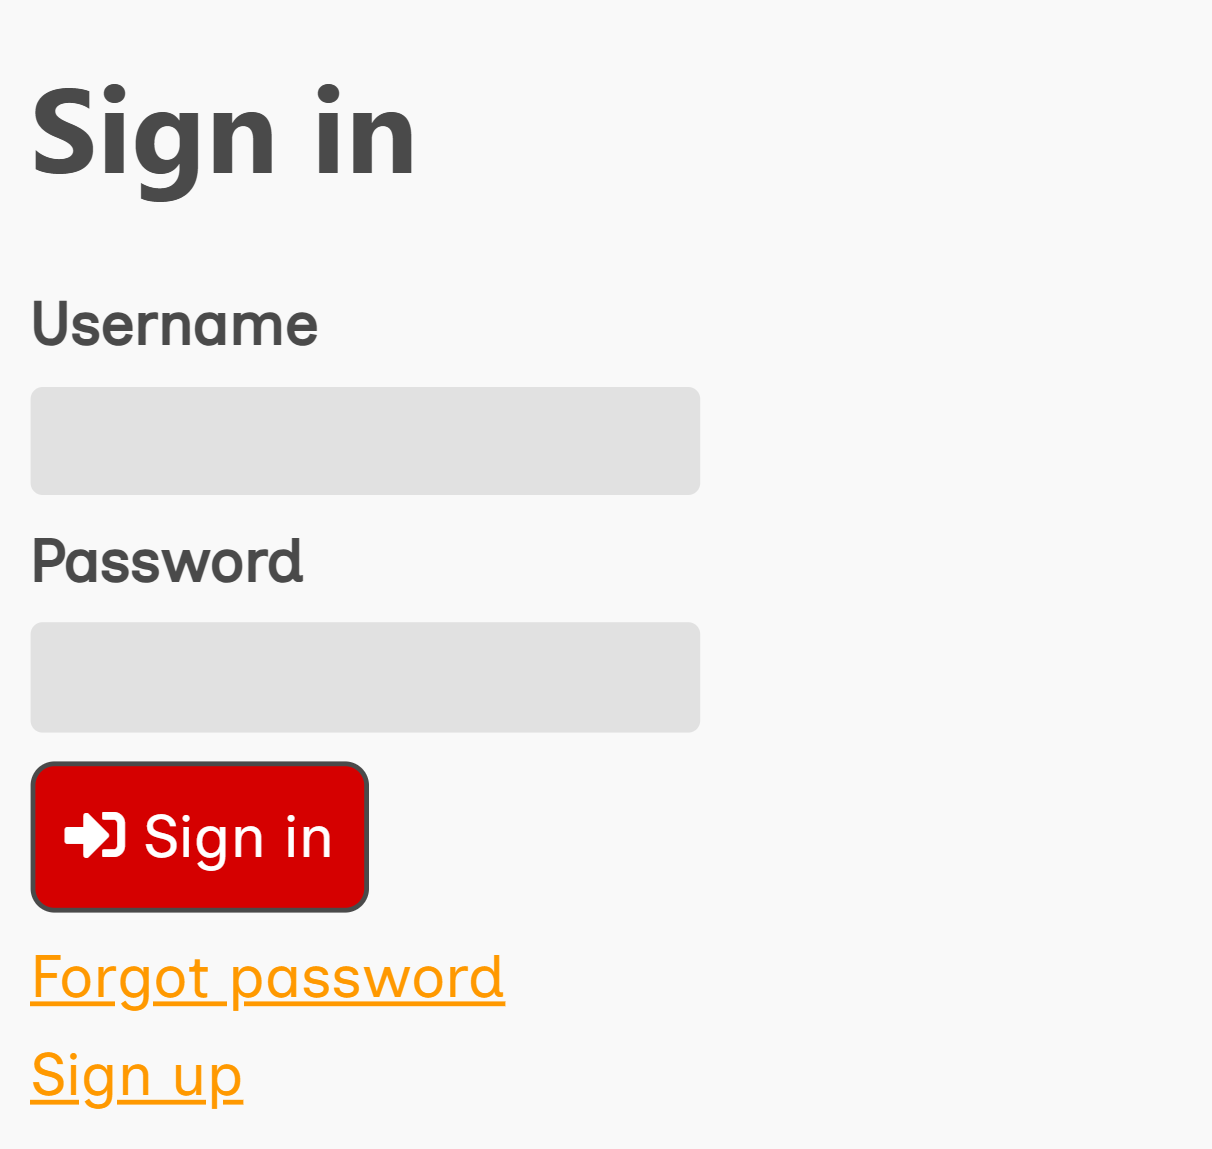
\includegraphics[width=0.45\textwidth]{assets/en/signin.png}
        \caption{Sign in page}
    \end{figure}

    Once signed in, you'll gain access to the \emph{homepage}.

    \begin{figure}[H]
        \centering
        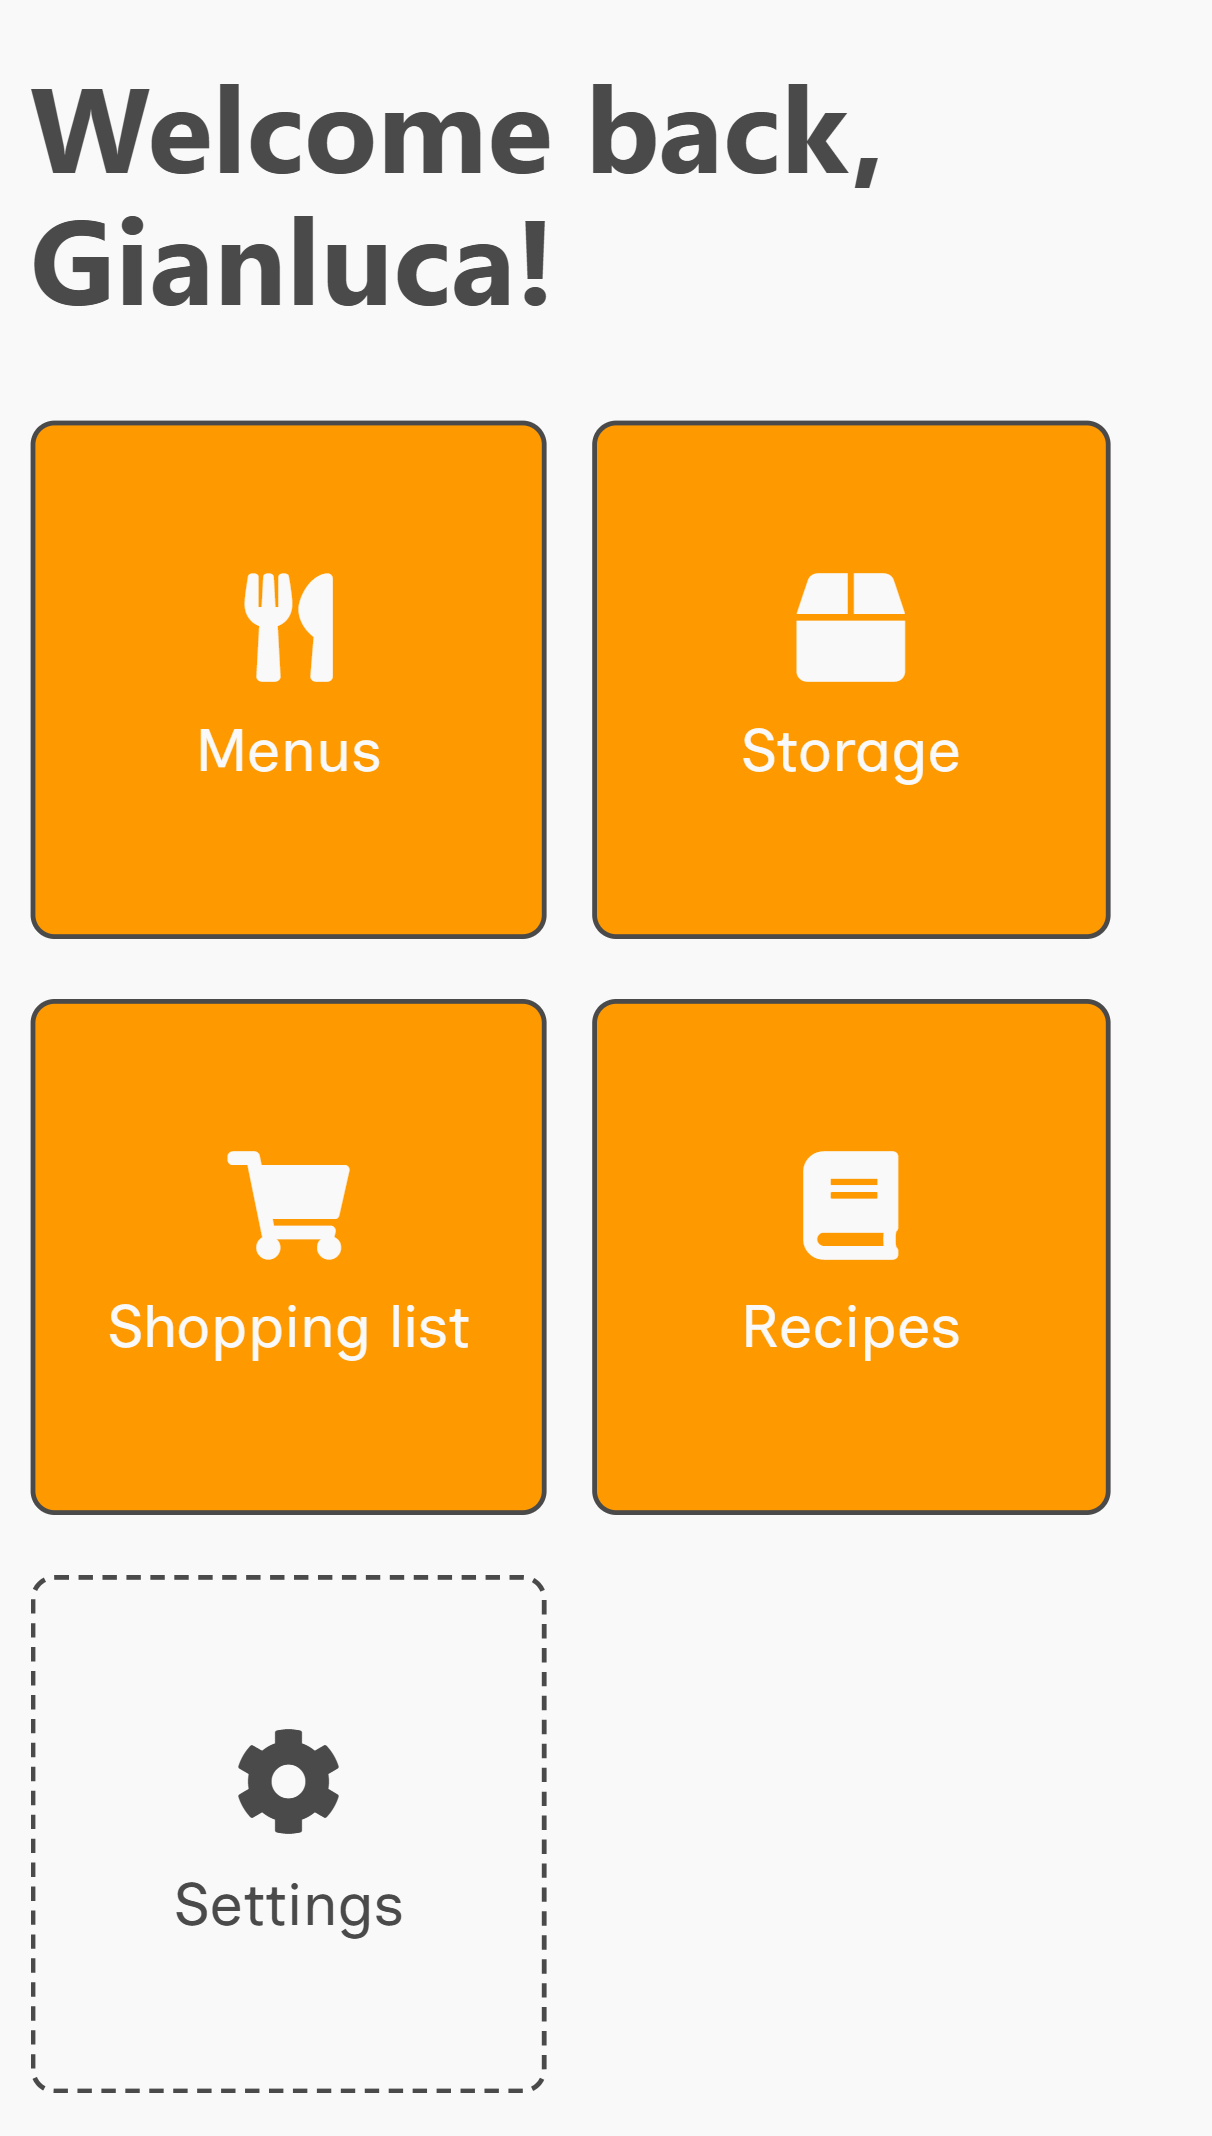
\includegraphics[width=0.45\textwidth]{assets/en/home.png}
        \caption{Home page}
    \end{figure}

    \section{Settings}

    The settings page contains a button to sign out, some buttons to change your username, email or password, and a button to permanently delete
    your account. There is also a button to change the language of the emails: in fact, you could also decide to see the website in a language, and
    receive your emails in another one.



    \chapter{Menus}

    A menu is composed of a name and 14 meals, two per day for a week.

    \section{Overview}

    From your homepage, with the \emph{Menus} button, you can see your menus and create new ones.

    \begin{figure}[H]
        \centering
        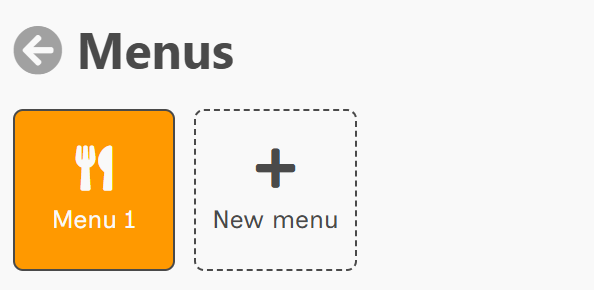
\includegraphics[width=0.45\textwidth]{assets/en/menus.png}
        \caption{The menus dashboard}
    \end{figure}

    Once clicked on a menu, you can see its content, and if you want edit or clone it. To delete it, you have to
    click the \emph{Edit} button first.

    \begin{figure}[H]
        \centering
        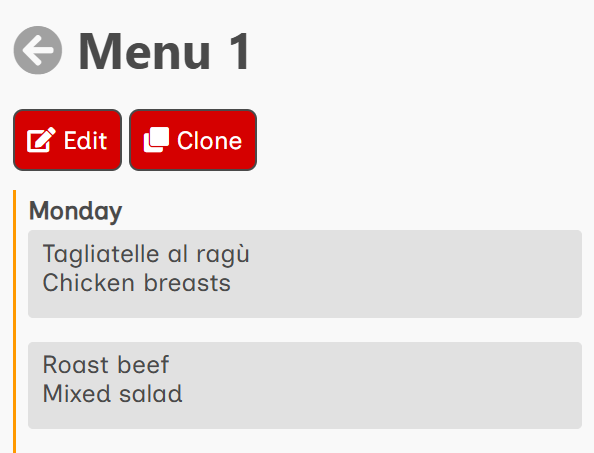
\includegraphics[width=0.45\textwidth]{assets/en/menu.png}
        \caption{A sample menu}
    \end{figure}



    \chapter{Storage}

    This is by far the most articulated part of CucinAssistant.
    Inside the storage, divided in sections, you can store articles, that are things you have in your kitchen, with a name,
    an optional expiration date and an optional quantity.

    \section{Sections}

    As said before, the articles can be grouped into sections, which you will see by clicking the \emph{Storage} button on
    your home page.

    \begin{figure}[H]
        \centering
        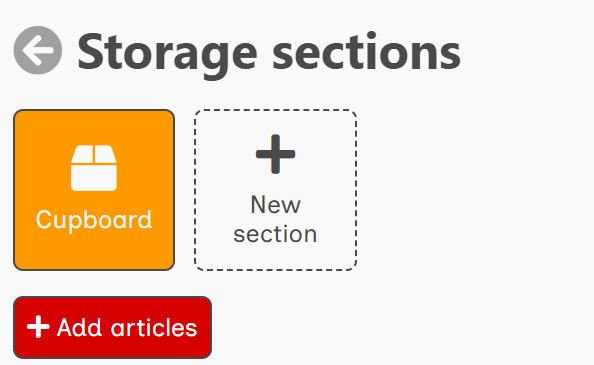
\includegraphics[width=0.45\textwidth]{assets/en/sections.png}
        \caption{The storage dashboard}
    \end{figure}

    You can create new sections with the button in the dashboard; to edit (or delete them) you have to open them and click the 
    \emph{Edit section} button.

    \section{Articles}

    You can see the articles of each section by clicking on it (and, if you want, search for a name).
    Articles are ordered by their expiration date; the expired ones will have a red band on the left, instead of the common orange one.

    \begin{figure}[H]
        \centering
        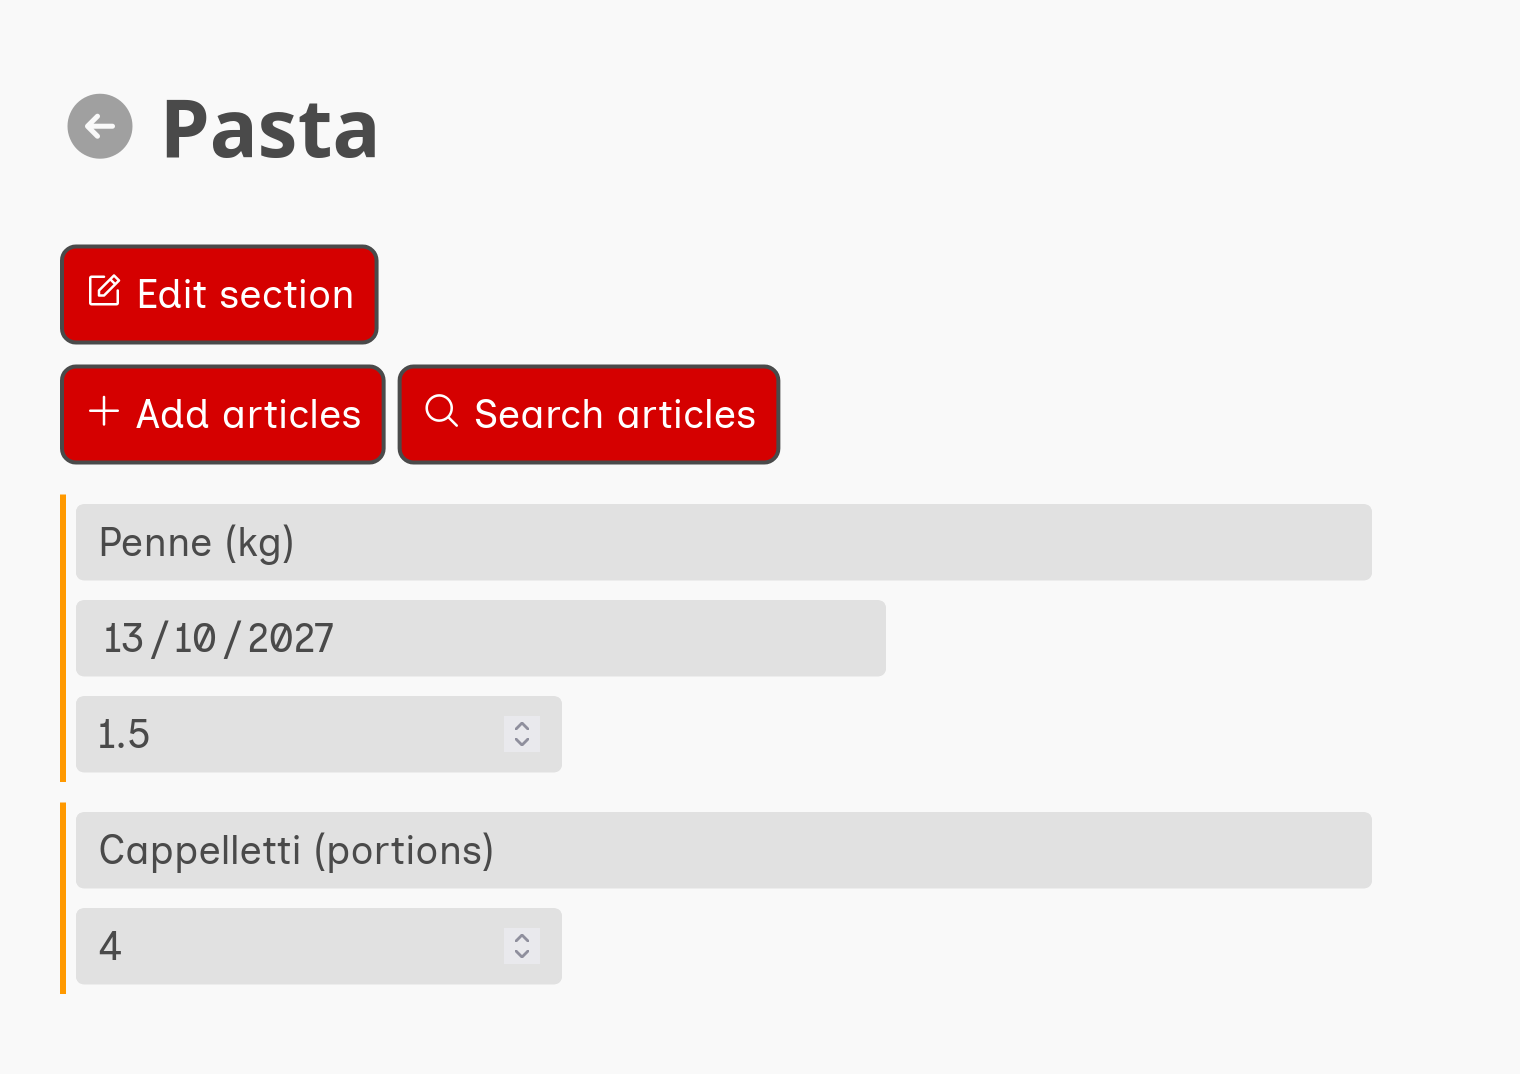
\includegraphics[width=0.45\textwidth]{assets/en/articles.png}
        \caption{An example section}
    \end{figure}

    You can add articles both from inside a section and outside a section; in the latter case, for each article added you'll also have
    to specify in which section to put each article.

    Remember that an article is identified by its name and expiration, so if you'll try to add an article that you already have in storage,
    CucinAssistant will add the quantities, and not create duplicates. On the other hand, if the expiration date differs, it will create another
    article.

    \section{Articles editing}

    To edit an article you have to click on it. After that, you'll see it alone, with some arrows (or blank buttons) and a \emph{Delete} button.
    The arrows button are there to make you scroll across each article in that section, in the same order of the list view.
    If you want to delete an article, you can simply click the button; if you want to edit it, you can do it directly: once something has changed,
    the three buttons will hide, and a \emph{Save} and \emph{Discard} buttons will be shown, so that you can confirm or not your changes and then
    proceed with the other articles.
    Note that if you change an expiration date, the order may change: in this case, you'll be redirected at the list view.

    \begin{figure}[H]
        \centering
        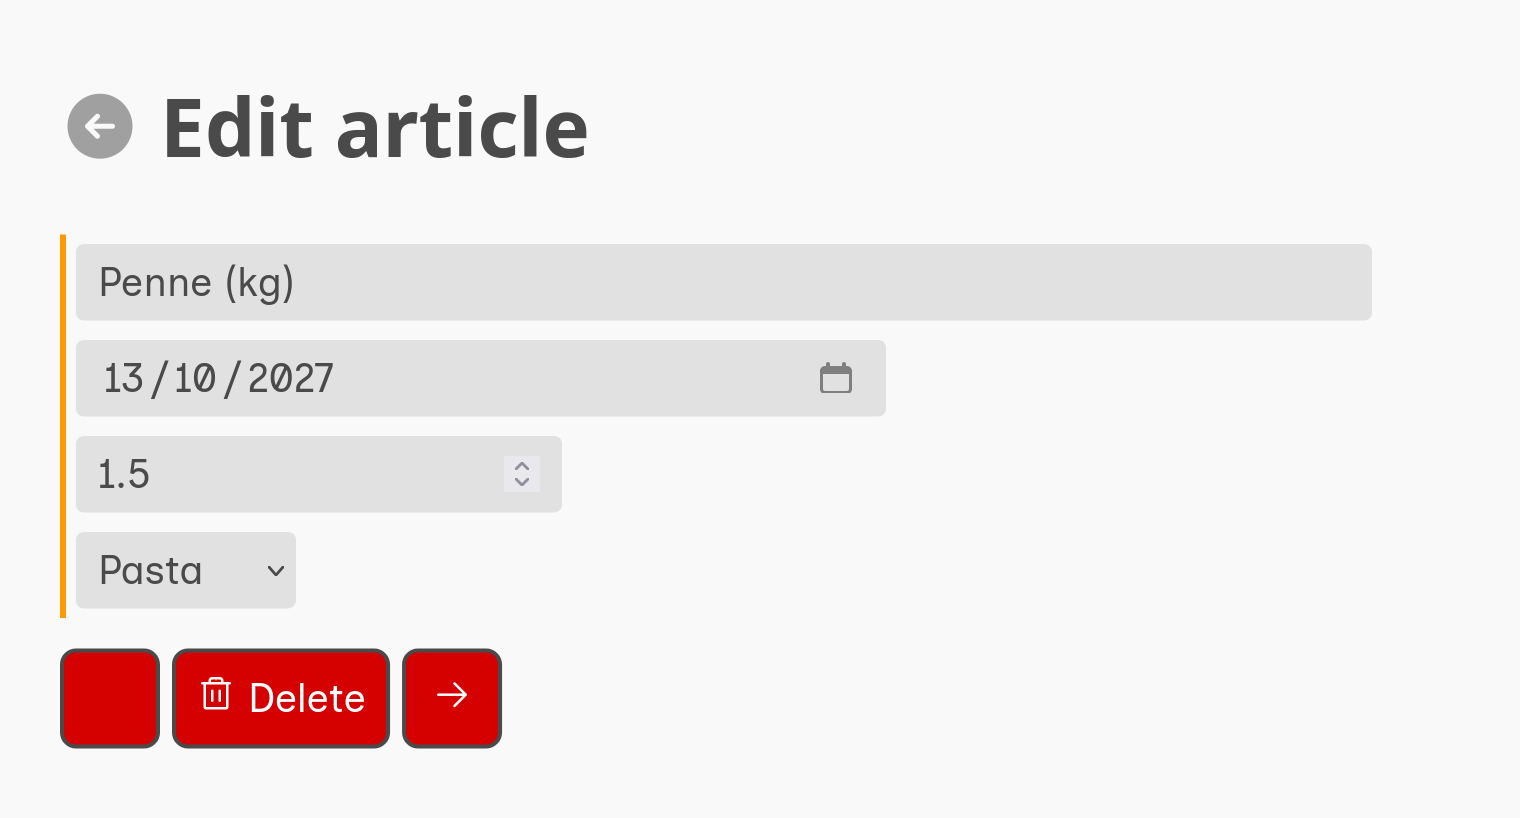
\includegraphics[width=0.45\textwidth]{assets/en/article.png}
        \caption{An example article being edited, before any changes}
    \end{figure}
\end{document}
